\chapter{Einleitung}
\label{cha:Einleitung}

\section{Zielsetzung}
Diese Bachelorarbeit dient als Vorarbeit für die Re-Implementierung einer existierenden Maillösung  der Frima curecomp GembH, wobei in dieser Arbeit der Fokus auf die Re-Implementierung des Designs gelegt wird. Diese Arbeit wird aufzeigen wie das existierende System in seinen Bereichen wie Client-API, Datenbank Integration und das Erstellen der E-Mails, in weitere Folge 'E-Mail Vorlagen' genannt, zurzeit funktioniert und designt wurde. Dieses existierende Design wird analysiert und ein Verbesserungsvorschlag eingebracht wie ein mögliches neues Design aussehen könnte. Die Konzepte der Implementierung wie die verwendeten Software Muster, die Grundlage der Designentscheidung sowie deren Vorteile und Nachteile werden in dieser Arbeit diskutiert. \\\\
Da meiner Meinung nach die existierende Implementierung einige Mängel und Designfehlentscheidungen beinhaltet und dadurch weder flexibel noch erweiterbar ist, wurde der Fokus dieser Arbeit auf das Design dieser Maillösung und dessen Verbesserung gesetzt, wobei diese Arbeit wiederum als Grundlage für die praktische Bachelorarbeit dienen soll, die die Umsetzung der hier entwickelten und diskutierten Konzepte beinhalten soll. \\\\
Als Unterstützung wurden folgende beiden literarischen Werke gewählt:
\begin{enumerate}
	\item Refactoring to patterns\footnote{Author: Joshua Kerhievsky, ISBN: 0-321-21335-1}
	\item Refactoring Databases\footnote{Author: Scott W.Ambler/Pramod J.Sadalage, ISBN: 0-321-29353-3} 
\end{enumerate}
\newpage

\section{Anforderungen}
Über die Zeit haben sich die Anforderungen an das Mailsystem derartig geändert, dass diese nicht mehr mit der existierenden Implementierung umgesetzt werden können. Dies liegt vor allem daran dass die existierende Implementierung aus dem Jahre 2002 stammt und man dessen umgesetztes Design mittlerweile vollständig ausgereizt hat. Andererseits muss man aber auch beachten dass die angeschlossenen Systeme sich über die Zeit evolutioniert, also weiterentwickelt, haben und daher auch neue Anforderungen stellen. Ebenso haben sich auch die Kundenanforderungen geändert.
\\
Aufgrund dieser Ausgangssituation wurden folgende technische Anforderungen definiert, die im folgenden aufgelistet sind.\\
\begin{itemize}
	\item Persistenz der versendeten E-Mails inklusive Anhänge.
	\item Integration in andere Systeme in Form von Rest-API (Rest-Service)
	\item Metadaten sollen für E-Mails definiert werden können (z.B.: Gruppierung)
	\item Konfigurierbarkeit des Mailversands, Speicherung, Archivierung, ...
\end{itemize}
\ \\
Das Gesamtsystem soll hierbei so flexibel wie möglich sein und muss in der Lage sein zumindest mit dem Systemen der Firma curecomp zu interagieren. 
\newpage

\section{Überblick Ist-System} 
Der jetzige Mailservice besteht im Grunde nur aus einer Konsolen Applikation, einigen Datenbank Tabellen, und den Implementierungen der DAO \emph{(Data-Access-Object)} der beiden angeschlossenen Systeme. Mann sieht einerseits dass hier die Redundanz in Form der DAO Implementierungen der angeschlossenen Systeme Inkonsistenz mit sich bringt und andererseits dass die Koppelung über die Datenbank unflexibel ist und alle angeschlossenen Systeme mit ihren eigenen Implementierungen darauf zugreifen und es kein übergeordnetes System gibt, welches die allgemeinen Aktionen weg abstrahiert, bündelt und allen Systemen zur Verfügung stellt. 
\\
\begin{figure}[h]
\centering
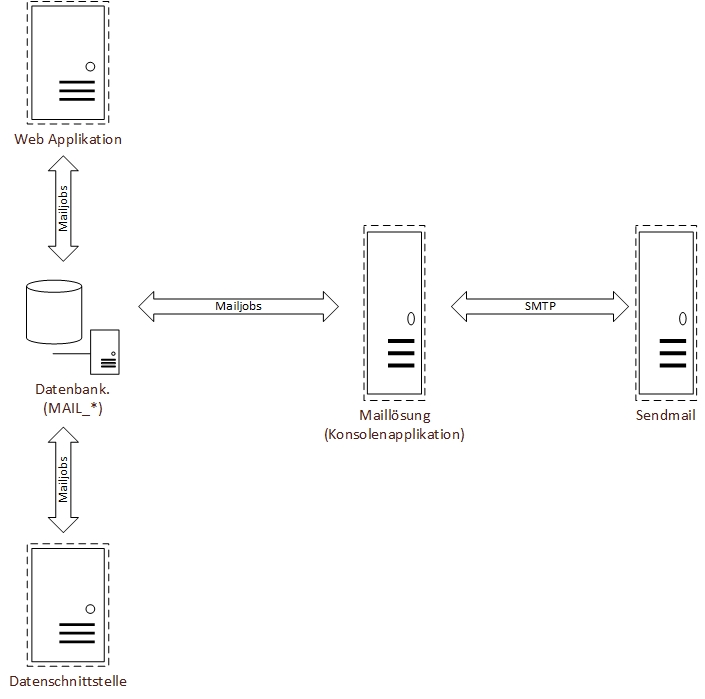
\includegraphics[scale=0.6]{Systemaufbau_alt.jpg} %{CS0031}
\caption{Diese Abbildung zeigt den konzeptionellen Aufbau der existierenden Maillösung und den jetzigen Kommunikationsweg zwischen den Systemteilnehmern}
\label{fig:systemaufbau-alt}
\end{figure}